\documentclass{article}
\usepackage[margin=1in]{geometry}
\usepackage{amsmath}
\usepackage{amsfonts}
\usepackage{graphicx}
% Calligraphic fonts
\newcommand{\calA}{{\cal A}}
\newcommand{\calB}{{\cal B}}
\newcommand{\calC}{{\cal C}}
\newcommand{\calD}{{\cal D}}
\newcommand{\calE}{{\cal E}}
\newcommand{\calF}{{\cal F}}
\newcommand{\calG}{{\cal G}}
\newcommand{\calH}{{\cal H}}
\newcommand{\calI}{{\cal I}}
\newcommand{\calJ}{{\cal J}}
\newcommand{\calK}{{\cal K}}
\newcommand{\calL}{{\cal L}}
\newcommand{\calM}{{\cal M}}
\newcommand{\calN}{{\cal N}}
\newcommand{\calO}{{\cal O}}
\newcommand{\calP}{{\cal P}}
\newcommand{\calQ}{{\cal Q}}
\newcommand{\calR}{{\cal R}}
\newcommand{\calS}{{\cal S}}
\newcommand{\calT}{{\cal T}}
\newcommand{\calU}{{\cal U}}
\newcommand{\calV}{{\cal V}}
\newcommand{\calW}{{\cal W}}
\newcommand{\calX}{{\cal X}}
\newcommand{\calY}{{\cal Y}}
\newcommand{\calZ}{{\cal Z}}

% Sets:
\newcommand{\setA}{\textsf{A}}
\newcommand{\setB}{\textsf{B}}
\newcommand{\setC}{\textsf{C}}
\newcommand{\setD}{\textsf{D}}
\newcommand{\setE}{\textsf{E}}
\newcommand{\setF}{\textsf{F}}
\newcommand{\setG}{\textsf{G}}
\newcommand{\setH}{\textsf{H}}
\newcommand{\setI}{\textsf{I}}
\newcommand{\setJ}{\textsf{J}}
\newcommand{\setK}{\textsf{K}}
\newcommand{\setL}{\textsf{L}}
\newcommand{\setM}{\textsf{M}}
\newcommand{\setN}{\textsf{N}}
\newcommand{\setO}{\textsf{O}}
\newcommand{\setP}{\textsf{P}}
\newcommand{\setQ}{\textsf{Q}}
\newcommand{\setR}{\textsf{R}}
\newcommand{\setS}{\textsf{S}}
\newcommand{\setT}{\textsf{T}}
\newcommand{\setU}{\textsf{U}}
\newcommand{\setV}{\textsf{V}}
\newcommand{\setW}{\textsf{W}}
\newcommand{\setX}{\textsf{X}}
\newcommand{\setY}{\textsf{Y}}
\newcommand{\setZ}{\textsf{Z}}

% Vectors
\newcommand{\bfa}{\mathbf{a}}
\newcommand{\bfb}{\mathbf{b}}
\newcommand{\bfc}{\mathbf{c}}
\newcommand{\bfd}{\mathbf{d}}
\newcommand{\bfe}{\mathbf{e}}
\newcommand{\bff}{\mathbf{f}}
\newcommand{\bfg}{\mathbf{g}}
\newcommand{\bfh}{\mathbf{h}}
\newcommand{\bfi}{\mathbf{i}}
\newcommand{\bfj}{\mathbf{j}}
\newcommand{\bfk}{\mathbf{k}}
\newcommand{\bfl}{\mathbf{l}}
\newcommand{\bfm}{\mathbf{m}}
\newcommand{\bfn}{\mathbf{n}}
\newcommand{\bfo}{\mathbf{o}}
\newcommand{\bfp}{\mathbf{p}}
\newcommand{\bfq}{\mathbf{q}}
\newcommand{\bfr}{\mathbf{r}}
\newcommand{\bfs}{\mathbf{s}}
\newcommand{\bft}{\mathbf{t}}
\newcommand{\bfu}{\mathbf{u}}
\newcommand{\bfv}{\mathbf{v}}
\newcommand{\bfw}{\mathbf{w}}
\newcommand{\bfx}{\mathbf{x}}
\newcommand{\bfy}{\mathbf{y}}
\newcommand{\bfz}{\mathbf{z}}


\newcommand{\bfalpha}{\boldsymbol{\alpha}}
\newcommand{\bfbeta}{\boldsymbol{\beta}}
\newcommand{\bfgamma}{\boldsymbol{\gamma}}
\newcommand{\bfdelta}{\boldsymbol{\delta}}
\newcommand{\bfepsilon}{\boldsymbol{\epsilon}}
\newcommand{\bfzeta}{\boldsymbol{\zeta}}
\newcommand{\bfeta}{\boldsymbol{\eta}}
\newcommand{\bftheta}{\boldsymbol{\theta}}
\newcommand{\bfiota}{\boldsymbol{\iota}}
\newcommand{\bfkappa}{\boldsymbol{\kappa}}
\newcommand{\bflambda}{\boldsymbol{\lambda}}
\newcommand{\bfmu}{\boldsymbol{\mu}}
\newcommand{\bfnu}{\boldsymbol{\nu}}
\newcommand{\bfomicron}{\boldsymbol{\omicron}}
\newcommand{\bfpi}{\boldsymbol{\pi}}
\newcommand{\bfrho}{\boldsymbol{\rho}}
\newcommand{\bfsigma}{\boldsymbol{\sigma}}
\newcommand{\bftau}{\boldsymbol{\tau}}
\newcommand{\bfupsilon}{\boldsymbol{\upsilon}}
\newcommand{\bfphi}{\boldsymbol{\phi}}
\newcommand{\bfchi}{\boldsymbol{\chi}}
\newcommand{\bfpsi}{\boldsymbol{\psi}}
\newcommand{\bfomega}{\boldsymbol{\omega}}
\newcommand{\bfxi}{\boldsymbol{\xi}}
\newcommand{\bfell}{\boldsymbol{\ell}}

% Matrices
\newcommand{\bfA}{\mathbf{A}}
\newcommand{\bfB}{\mathbf{B}}
\newcommand{\bfC}{\mathbf{C}}
\newcommand{\bfD}{\mathbf{D}}
\newcommand{\bfE}{\mathbf{E}}
\newcommand{\bfF}{\mathbf{F}}
\newcommand{\bfG}{\mathbf{G}}
\newcommand{\bfH}{\mathbf{H}}
\newcommand{\bfI}{\mathbf{I}}
\newcommand{\bfJ}{\mathbf{J}}
\newcommand{\bfK}{\mathbf{K}}
\newcommand{\bfL}{\mathbf{L}}
\newcommand{\bfM}{\mathbf{M}}
\newcommand{\bfN}{\mathbf{N}}
\newcommand{\bfO}{\mathbf{O}}
\newcommand{\bfP}{\mathbf{P}}
\newcommand{\bfQ}{\mathbf{Q}}
\newcommand{\bfR}{\mathbf{R}}
\newcommand{\bfS}{\mathbf{S}}
\newcommand{\bfT}{\mathbf{T}}
\newcommand{\bfU}{\mathbf{U}}
\newcommand{\bfV}{\mathbf{V}}
\newcommand{\bfW}{\mathbf{W}}
\newcommand{\bfX}{\mathbf{X}}
\newcommand{\bfY}{\mathbf{Y}}
\newcommand{\bfZ}{\mathbf{Z}}


\newcommand{\bfGamma}{\boldsymbol{\Gamma}}
\newcommand{\bfDelta}{\boldsymbol{\Delta}}
\newcommand{\bfTheta}{\boldsymbol{\Theta}}
\newcommand{\bfLambda}{\boldsymbol{\Lambda}}
\newcommand{\bfPi}{\boldsymbol{\Pi}}
\newcommand{\bfSigma}{\boldsymbol{\Sigma}}
\newcommand{\bfUpsilon}{\boldsymbol{\Upsilon}}
\newcommand{\bfPhi}{\boldsymbol{\Phi}}
\newcommand{\bfPsi}{\boldsymbol{\Psi}}
\newcommand{\bfOmega}{\boldsymbol{\Omega}}


% Blackboard Bold:
\newcommand{\bbA}{\mathbb{A}}
\newcommand{\bbB}{\mathbb{B}}
\newcommand{\bbC}{\mathbb{C}}
\newcommand{\bbD}{\mathbb{D}}
\newcommand{\bbE}{\mathbb{E}}
\newcommand{\bbF}{\mathbb{F}}
\newcommand{\bbG}{\mathbb{G}}
\newcommand{\bbH}{\mathbb{H}}
\newcommand{\bbI}{\mathbb{I}}
\newcommand{\bbJ}{\mathbb{J}}
\newcommand{\bbK}{\mathbb{K}}
\newcommand{\bbL}{\mathbb{L}}
\newcommand{\bbM}{\mathbb{M}}
\newcommand{\bbN}{\mathbb{N}}
\newcommand{\bbO}{\mathbb{O}}
\newcommand{\bbP}{\mathbb{P}}
\newcommand{\bbQ}{\mathbb{Q}}
\newcommand{\bbR}{\mathbb{R}}
\newcommand{\bbS}{\mathbb{S}}
\newcommand{\bbT}{\mathbb{T}}
\newcommand{\bbU}{\mathbb{U}}
\newcommand{\bbV}{\mathbb{V}}
\newcommand{\bbW}{\mathbb{W}}
\newcommand{\bbX}{\mathbb{X}}
\newcommand{\bbY}{\mathbb{Y}}
\newcommand{\bbZ}{\mathbb{Z}}





\title{ECE 417 Midterm 1}
\date{Feb 18th, 2021}
\author{Vikas Dhiman}

\newtheorem{prob}{Problem}
\newif\ifsol
\solfalse

\begin{document}
\maketitle

\begin{tabular}{p{0.5\linewidth}p{0.5\linewidth}}
  (1) Student name:& Student email: \\
\end{tabular}

\subsubsection*{About the exam}
\begin{enumerate}
  \item There are total 5 problems. You must attempt all 5. 
  \item Maximum marks: 50 (70 with bonus).
  \item Maximum time allotted:  50 min
  \item Calculators are allowed.
  \item One US Letter size or A4 size cheat sheet (both-sides) is allowed.
\end{enumerate}

\begin{prob}
  What are the two criteria for a $3 \times 3$ matrix $A$ to be a valid rotation matrix?
  (5 min, 5 marks)
\end{prob}
\newpage

\begin{prob}
  For Fig~\ref{fig:rot-2D}, write the rotation matrix $R(\theta)$ that converts
  between coordinates of point from red coordinate frame $\bfp_c$ to green
  coordinate frame $\bfp_w$ such that $\bfp_w = R(\theta) \bfp_c$. (Optional
  part) Test your
  formula if it looks correct for $\theta  = -30^\circ$, $\bfp_c
  = \begin{bmatrix} 1 \\ 3 \end{bmatrix}$.
  (5 min, 5 marks)
\end{prob}

\begin{figure}
  \centering
  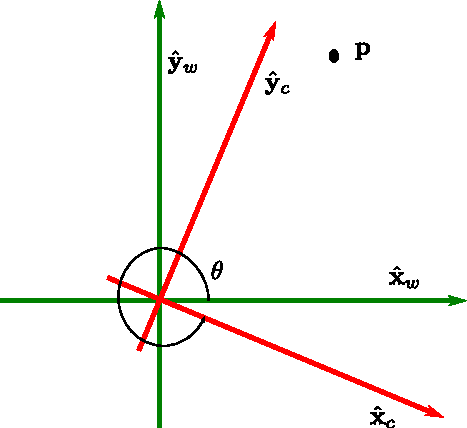
\includegraphics[width=0.5\linewidth]{media/rot-2D.pdf}
  \caption{Rotation between red frame and green coordinate frame.}
  \label{fig:rot-2D}
\end{figure}

\newpage

\begin{prob}
  In Figure~\ref{fig:Rodrigues-formula}, we are rotating point $\bfv$ around
  axis unit-vector $\hat{\bfk}$ by an angle $\theta$. $\bfv_{\perp}$ lies in the plane of $\bfv$
  and $\hat{\bfk}$ and is orthogonal (perpendicular) to $\bfk$. $\bfw$ is
  perpendicular to the plane of $\bfv$ and $\hat{\bfk}$. First, write the
  unit-vector $\hat{\bfw}$ in terms of $\bfv$ and $\hat{\bfk}$.
  Then write unit-vector $\hat{\bfv}_\perp$ in terms of $\bfv$ and $\hat{\bfk}$.
  (10 min, 10 marks)
\end{prob}
\begin{figure}
  \centering
  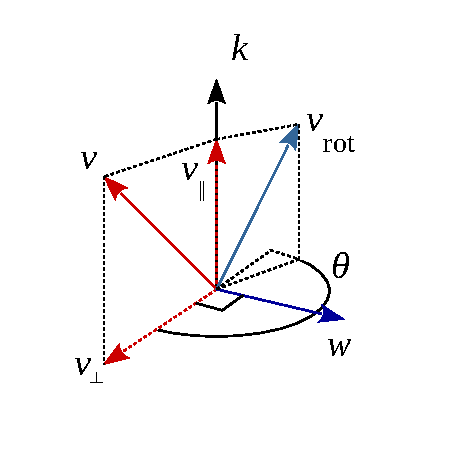
\includegraphics[width=0.5\linewidth]{media/Rodrigues-formula.pdf}
  \caption{Rotation of point $\bfv$ around axis $\bfk$ by angle $\theta$}
  \label{fig:Rodrigues-formula}
\end{figure}

\newpage
\begin{prob}
  Using the fact that at minima (or maxima) of a differentiable function
  $f(\bfx)$, $\nabla_\bfx f(\bfx) = 0$, find the minima of the following
  function,
  \begin{align}
    f(\bfx) = (\bfx - \bfp)^\top A^\top A (\bfx-\bfp) + 2 \bfb^\top \bfx + c,
  \end{align}
  where $\bfx \in \bbR^n$, $\bfp \in \bbR^n$, $\bfb \in \bbR^n$, $c \in \bbR$,
  $A \in \bbR^{m \times n}$. Assume $A^\top A$ to be invertible.
  (10 min, 10 marks)
\end{prob}

\newpage

\begin{prob}
  In figure~\ref{fig:image-road-triangulation} find the 3D position of mercedes logo
  in the World coordinate frame, in terms of $h$ (the height of the camera),
  image-coordinates of the mercedes logo $\bfu$, camera matrix $K$, and $h_2$
  the height of logo from the road. The Camera mounted directly on top of the
world frame. The road is a perfect plane and the pothole lies on the road plane
(Equation of plane $Z_w = 0$ in the world coordinate frame). You do not need to
substitute in the values, providing a formula or pseudo-code for computing the
pothole coordinates is enough. (20 min, 20 marks, Bonus marks: 20)
\end{prob}

\begin{figure}
  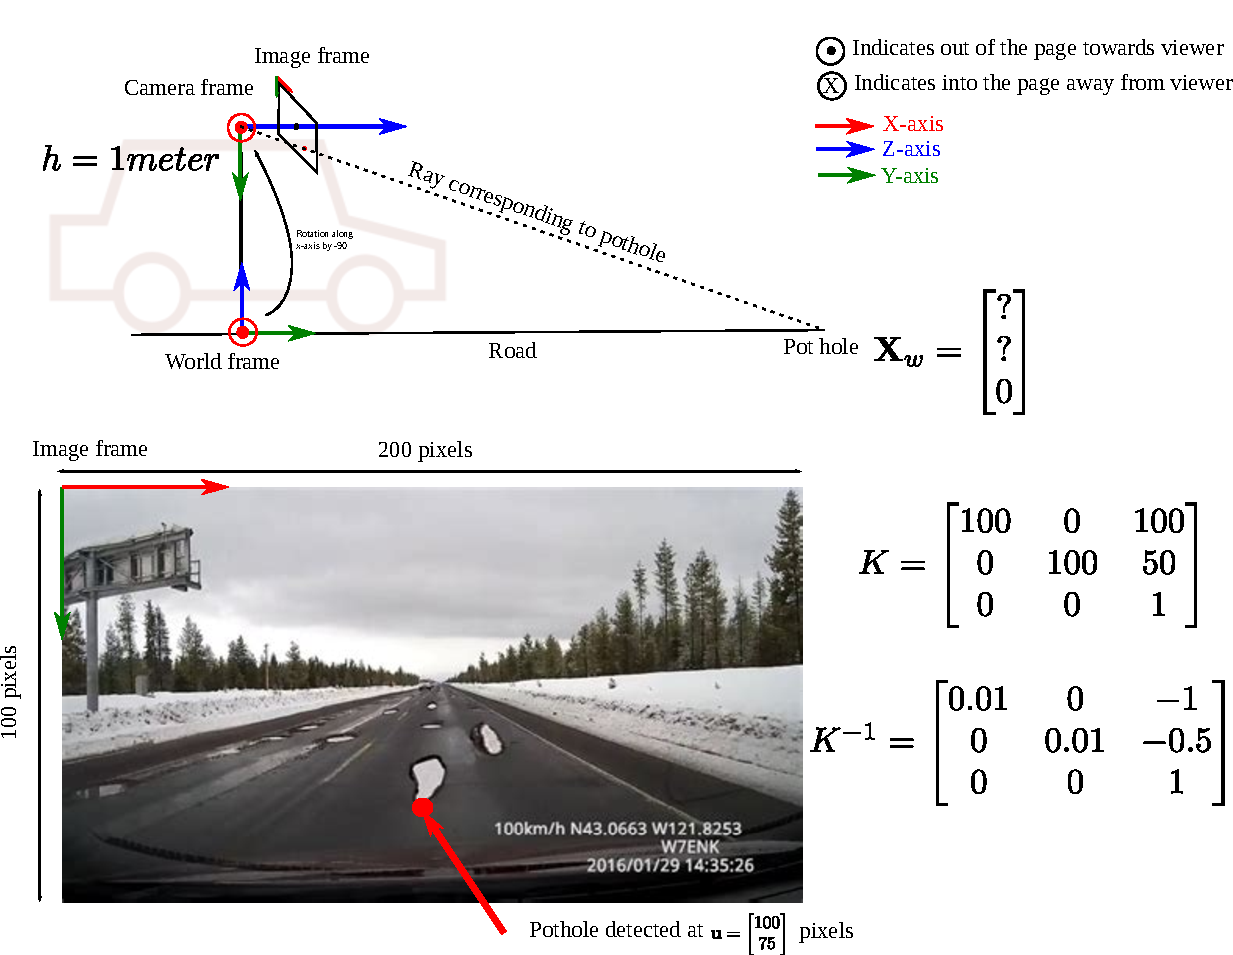
\includegraphics[width=\linewidth]{media/image-road-triangulation.pdf}
  \caption{Image road triangulation}
  \label{fig:image-road-triangulation}
\end{figure}


\end{document}
